\documentclass[b5paper,11pt,oneside,fleqn]{article}
\usepackage{amsmath,amsthm,amssymb}

\usepackage{graphicx}
\usepackage{geometry}
\usepackage{xifthen}

\title{\raggedleft\sffamily\Huge fluid}
\author{\sffamily\itshape Bacco, Giacomo}
\date{}

\newcommand{\eu}{\mathrm{e}}
\newcommand{\je}{\mathrm{j}}

\newcommand{\ped}[1]{_\textup{#1}}
\newcommand{\ap}[1]{^\textup{#1}}
\newcommand{\pt}[1]{\mathsf{#1}}
\newcommand{\te}{\vartheta}

% magnet width
\newcommand{\wm}[1][]{%
w_{\textup{m}
\ifthenelse{\isempty{#1}{}}{}{,#1}%
}}
% flux-carrier width
\newcommand{\wc}[1][]{%
w_{\textup{c}
\ifthenelse{\isempty{#1}{}}{}{,#1}%
}}
% flux-barrier thickness
\newcommand{\tb}[1][]{%
t_{\textup{b}
\ifthenelse{\isempty{#1}{}}{}{,#1}%
}}
% iron rib width
\newcommand{\wrib}[1][]{%
w_{\textup{rib}
\ifthenelse{\isempty{#1}{}}{}{,#1}%
}}
% tangential iron rib width
\newcommand{\wribt}{\wrib[\text{t}]}
\newcommand{\xth}[1]{$ #1 $-th}
% flux-barrier angle
\newcommand{\ab}[1][]{%
\alpha_{\textup{b}
\ifthenelse{\isempty{#1}{}}{}{,#1}%
}}

\newcommand{\pih}[1][]{\tfrac{\pi}{2#1}}
\newcommand{\map}{\mathcal{M}}
\newcommand{\de}{\partial}

\usepackage{url}
\usepackage{hyperref}

\newcommand{\nonfinito}{\emph{to be continued\ldots}}

\begin{document}
\maketitle


\section*{Citing}
Please cite this work if you have used it in your project or in your program.
\vspace{0\baselineskip}

{\small\noindent%
Giacomo Bacco, \emph{fluid: Free Fluid Flux-Barriers Rotor for Synchronous 
Reluctance Motor Drawing}, GitHub, 2018, available at:
\url{https://github.com/gbacco5/fluid}
}


\tableofcontents



\section{Flow past a cylinder}

Let $ \rho_0 $ be the radius of the cylinder, $ \rho,\xi $ the polar coordinate
system in use.
One possible solution of this problem have these potential and streamline
functions:
\begin{align}
\phi(\rho,\xi) &= \left( \rho + \frac{\rho_0^2}{\rho} \right) \cos\xi \\[1ex]
\psi(\rho,\xi) &= \left( \rho - \frac{\rho_0^2}{\rho} \right) \sin\xi
\end{align}
Although these equations are deeply coupled, the radius $ \rho $ and the phase
$ \xi $ can be obtained as a function of the other quantities.
For our purposes, we use $ \psi $.
\begin{align}
\rho(\psi,\xi) &= \frac{\psi + \sqrt{\psi^2 + 4\rho_0^2 \sin^2\xi}}{2\sin\xi}
\\[1ex]
\xi(\psi,\rho) &= \arcsin \left( \frac{\rho\, \psi}{\rho^2 - \rho_0^2} \right)
\end{align}

The velocity field can also be derived through
\begin{equation}
\begin{aligned}
v_\rho(\rho,\xi)  &= \frac{\de\phi}{\de\rho} =
           \left( 1 - \frac{\rho_0^2}{\rho^2} \right) \cos\xi \\[1ex]
v_\xi(\rho,\xi)  &= \frac{1}{\rho} \frac{\de\phi}{\de\xi}  =
          -\left( 1 + \frac{\rho_0^2}{\rho^2} \right) \sin\xi
\end{aligned}
\end{equation}




\section{Conformal mapping}
From the reference plane, which is equivalent to a two-pole machine,
we use a complex map to obtain the quantities in the actual plane.
Let $ p $ be the number of pole pairs. Then:
\begin{equation}
\begin{aligned}
\zeta              &\xrightarrow{\;\map\;} z = \sqrt[p]{\zeta} \\
\rho\,\eu^{\je\xi} &\xrightarrow{\;\map\;}
                       r \, \eu^{\je\te} = \sqrt[p]{\rho}\,\eu^{\je
                       \xi/p} \\
\chi + \je\eta     &\xrightarrow{\;\map\;} x + \je y
\end{aligned}
\end{equation}
%
It is easy to find the inverse map:
\begin{equation}
\map\colon \sqrt[p]{\cdot} \qquad
\map^{-1}\colon (.)^p
\end{equation}

In the transformed plane, the velocities have a different expression:
\begin{equation}
\begin{aligned}
v_r(r,\te)  &=
p \left( r^{p-1} - \frac{R_0^{2p}}{r^{p+1}} \right) \cos p\te \\[1ex]
v_\te(r,\te)  &=
-p \left( r^{p-1} + \frac{R_0^{2p}}{r^{p+1}} \right) \sin p\te
\end{aligned}
\end{equation}
%
This vector field is tangent to the streamlines in every point in the
transformed plane. In order to work with this field in $ x,y $ coordinates, we
need a rotational map:
\begin{equation}
\begin{aligned}
v_x(r,\te) &= v_r \cos\te - v_\te \sin\te \\
v_\te(r,\te) &= v_r \sin\te + v_\te \cos\te
\end{aligned}
\end{equation}



\section{Computation of flux-barrier base points}

Refer to \autoref{fig: flux-barrier base points} for the points naming scheme.
Keep in mind that $ \pt{A}' $ is not simply the projection of $ \pt{A} $ onto 
the $ q $-axis, but it represent the original starting point for the barrier 
sideline, so it lies on the flux-barrier streamline. The same is true for 
points
$ \pt{B}',\pt{B} $, 
$ \pt{C}',\pt{C} $, and
$ \pt{D}',\pt{D} $.

\begin{figure}[tb]
\centering
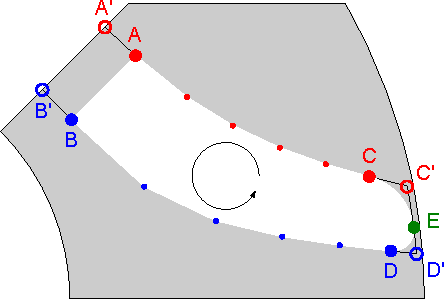
\includegraphics[width=0.75\linewidth]{gfx/BarrierPoints/BarrierPoints}
\caption{Flux-barrier base points description.}
\label{fig: flux-barrier base points}
\end{figure}

Let the flux-barrier and flux-carrier thicknesses be given.
Then the base points for the flux-barriers can be computed easily.
Let
$ D\ped{r} $ be the rotor outer diameter,
$ \wribt $ the tangential iron rib width,
$ \wc[k] $ the \xth{k} flux-carrier width,
and $ \tb[k] $ the \xth{k} flux-barrier thickness.%
\footnote{%
You may wonder why the main dimensions of the flux-carrier and
flux-barrier differ in the name (width versus thickness).
This is due to a choice of mine,
because I prefer to refer to width when the flux flows perpendicularly to the
dimension,
and to thickness when it flows in parallel.%
}
%
Then
\begin{equation}
\begin{aligned}
R\ped{r} &= \frac{D\ped{r}}{2} - \wribt \\
R_\pt{A_1'} &= R\ped{r} - \wc[1] \\
R_\pt{B_1'} &= R_\pt{A_1'} - \tb[1] \\
    &\:\:\,\vdots
\end{aligned}
\end{equation}
where $ R $ represents the radius from the origin.
%
So, in general:
\begin{equation}
\begin{aligned}
R_\pt{A_k'} &= R_\pt{B_{k-1}'} - \wc[k] \\
R_\pt{B_k'} &= R_\pt{A_{k-1}'} - \tb[k]
\end{aligned}
\end{equation}
with the exception $ R_\pt{B_0'} = R\ped{r} $.

Now we know both the radii and the angle -- always $ \pi/(2p) $ -- of the
flux-barrier internal points. So we can compute their respective streamline
value.



\subsection{Magnet insertion}
\[
\wrib[k] = \wrib[k] + \wm[k]
\]
where $ \wm[k] $ is the \xth{k} magnet width.


\subsection{Central base points}
We refer to points $ \pt{A} $ and $ \pt{B} $.
If the rib width is zero
$ \pt{A} \equiv \pt{A}' $ and
$ \pt{B} \equiv \pt{B}' $.

The line describing the $ q $-axis is
\begin{equation}
\begin{aligned}
y &= m x + q \\
m &= \tan\frac{\pi}{2p} \\
q &= \frac{\wrib}{2 \cos\frac{\pi}{2p}}
\end{aligned}
\end{equation}

\begin{equation}
\begin{cases}
y_\pt{A} - m x_\pt{A} - q = 0 \\
x_\pt{A} - r_\pt{A}(\psi_\pt{A'},\te_\pt{A}) \cos\te_\pt{A} = 0 \\
y_\pt{A} - r_\pt{A}(\psi_\pt{A'},\te_\pt{A}) \sin\te_\pt{A} = 0 \\
\end{cases}
\end{equation}
where $ \te_\pt{A} $ is used as the third degree of freedom and $ r_\pt{A} $ is
then a function of it.
The solution of such system can be determined solving the single equation
\begin{equation}
r_\pt{A}(\psi_\pt{A'},\te_\pt{A})
\bigl( \sin\te_\pt{A} - m \cos\te_\pt{A} \bigr) - q = 0
\end{equation}
in the unknown $ \te_\pt{A} $.
The function $ r(\psi,\te) $ is simply
\[
r(\psi,\te) = \sqrt[p]{ \rho(\psi,\te/p) \bigr) }
\]

The same equation can be written for point $ \pt{B} $ with the proper
substitution and repeated for all the flux-barriers.



\section{Outer base points}
We refer to points $ \pt{C} $, $ \pt{D} $, and $ \pt{E} $.
If the flux-barrier angle, $ \ab $, is given, then
\begin{equation}
\begin{aligned}
x_\pt{E} &= R_r \cos(\pih[p] - \ab) \\
y_\pt{E} &= R_r \sin(\pih[p] - \ab)
\end{aligned}
\end{equation}

Points $ \pt{C} $ and $ \pt{D} $ results from the connection of the
flux-barrier sidelines and point $ \pt{E} $.
This connection should be as smooth as possible in order to
avoid dangerous mechanical stress concentrations.
We are going to use circular arcs to make this connection.
So we impose the tangency between the flux-barrier sideline and the arc,
between the arc and the radius through point $ \pt{E} $.
The tangent to the sideline can be obtained through the velocity field
described above.

Then we want point $ \pt{C} $ to lay on the flux-barrier sideline. These
conditions represent a nonlinear system of 4 equations, in 6 unknowns.
So we need two more equations, which are that points $ \pt{C} $ and $ \pt{E} $
belong to the fillet circle with radius $ R $.
\begin{equation}
\begin{cases}
x_\pt{C} - r_\pt{C}(\psi_\pt{C}, \te_\pt{C}) \cos\te_\pt{C} = 0 \\
y_\pt{C} - r_\pt{C}(\psi_\pt{C}, \te_\pt{C}) \sin\te_\pt{C} = 0 \\
%
(x_\pt{C} - x_\pt{O_\pt{C}})^2 + (y_\pt{C} - y_\pt{O_\pt{C}})^2
- R_\pt{EC}^2 = 0 \\
(x_\pt{E} - x_\pt{O_\pt{C}})^2 + (y_\pt{E} - y_\pt{O_\pt{C}})^2
- R_\pt{EC}^2 = 0 \\
%
(x_\pt{O_\pt{C}} - x_\pt{E}) y_\pt{E} -
(y_\pt{O_\pt{C}} - y_\pt{E}) x_\pt{E} = 0 \\
%
(x_\pt{O} - x_\pt{C}) v_x(r_\pt{C},\te_\pt{C}) +
(y_\pt{O} - y_\pt{C}) v_y(r_\pt{C},\te_\pt{C})
\end{cases}
\end{equation}

The very same system can be written and solved for point $ \pt{D} $.



\section{Flux-barrier sideline points}

\nonfinito 



\section{Example of Matlab/Octave plot}

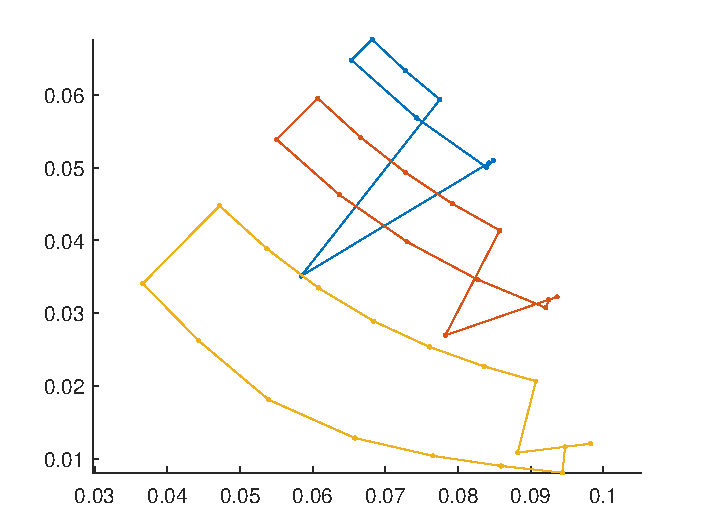
\includegraphics[width=0.75\linewidth]{gfx/MatlabOutput}

Here is an example of a Matlab/Octave output plot.
The V-shaped lines represent the radii of the fillet arcs, which were not worth 
to be shown in Matlab/Octave.




\end{document}
